\section{Related Work}
\label{sec:review}

This section provides a brief survey of salient forecasting architectures, from early rasterized and vectorized approaches to the current state-of-the-art transformer-based models.

\begin{figure}[H]
\centering
\begin{subfigure}[t]{0.35\textwidth}
    \centering
    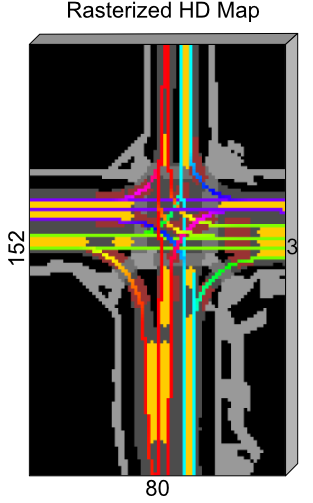
\includegraphics[width=\textwidth]{figures/caspnet-bev-repr.png}
    \label{fig:rasterized}
\end{subfigure}
\hfill
\begin{subfigure}[t]{0.37\textwidth}
    \centering
    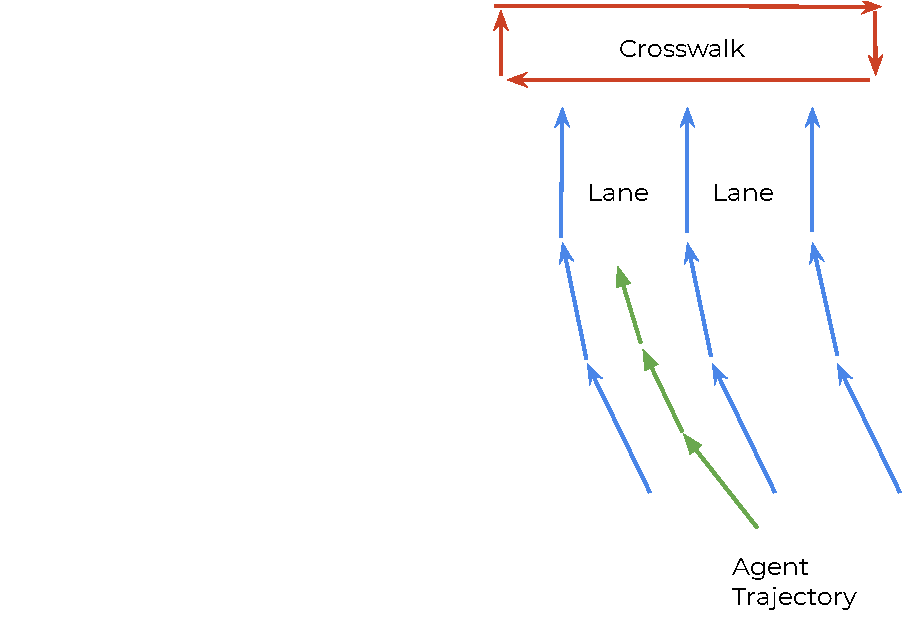
\includegraphics[width=\textwidth]{figures/vectornet-2020-vector-repr.pdf}
    \label{fig:vectorized}
\end{subfigure}
\caption{Scene representation paradigms: (a) rasterized BEV encoding~\cite{caspnetSchäfer2022}, (b) vectorized polyline preservation~\cite{gao2020vectornet}.}
\label{fig:scene_representations}
\end{figure}

\subsection{Rasterized Scene Representations}
Early approaches rasterized scenes into bird's-eye-view (BEV) images, applying CNNs to learn scene-representations~\cite{cui2019multimodal,chai2019multipath}. Static context is encoded as \(\mathbf{I}_s \in \mathbb{R}^{C \times H \times W}\), while dynamic elements are expressed as stacks over \(T_p\) timesteps.

\textbf{CASPNet}~\cite{caspnetSchäfer2022} processes rasterised \emph{dynamic} (BEV trajectory stack) and \emph{static} (HD-map RGB) inputs through two \emph{symmetric} encoder pyramids. The trajectory branch is a four-stage CNN down-sampling cascade, whereas the map branch swaps the first two \(3{\times}3\) kernels for \emph{Gabor CNN blocks}~\cite{jiang2017gabor} to provide steerable orientation-scale filters well aligned with elongated lane markings. At every resolution level~\(\ell\!\in\!\{0,\dots,3\}\) a ConvLSTM cell integrates the \(T_p\) history, producing multi-scale feature maps \(F_\ell\!\in\!\mathbb{R}^{C_\ell\times H_\ell\times W_\ell}\). The encoder therefore outputs the \textbf{scene representation}
\begin{equation}
\label{eq:caspnet_scene_repr}
\mathcal{F}
  \;=\;
  \bigl\{\,F_{0},\,F_{1},\,F_{2},\,F_{3}\bigr\},
\qquad
F_{\ell}\in\mathbb{R}^{C_{\ell}\times H_{\ell}\times W_{\ell}},
\end{equation}

which is fed into the decoder via \emph{lateral skip connections}, heavily resembling the famous U-Net architecture.

The grid-based decoder employs residual up-sampling blocks (similar to a U-Net decoder) to predict joint occupancy and offset heat-maps for every agent, preserving constant inference cost regardless of agent. Finally, a ConvLSTM ``unfolds'' the up-scaled heat-maps onto \( T_f \) future time steps.

\textbf{CASPFormer}~\cite{caspformerYadav2024} retains CASPNet's multi-scale CNN backbone to encode rasterized BEV inputs into hierarchical feature maps $\mathcal{F} = \{F_0, F_1, F_2, F_3\}$. These are flattened into tokens at each scale and enriched with 2D sinusoidal position embeddings before being passed into a \textbf{Deformable Self-Attention} layer that fuses multi-scale context efficiently at $\mathcal{O}(N)$ complexity~\cite{zhu2021deformabledetr}. The resulting fused tokens serve as the keys and values in the decoder.

The decoder recurrently predicts future trajectories via a \textbf{Deformable Cross-Attention} module. At each timestep, it uses two sets of learnable queries:
\begin{enumerate}
    \item \emph{temporal queries} that encode temporal dependencies across steps, and
    \item \emph{mode queries} that allow the model to specialize into $M$ diverse behavior patterns and combat mode collapse.
\end{enumerate}

These are summed element-wise to form the final decoder query which is used to predict both the attention weights and the sampling offsets for deformable attention, relative to a \emph{reference anchor point} (initially the ego pose).

The decoder updates the reference point in each iteration using the trajectory output of the previous step. The final trajectory positions $\boldsymbol{\mu}_t = (x, y)$ are generated through a shared \textbf{MLP head} that maps decoder outputs Cartesian coordinates as well \emph{mode logits} $\pi_k$ and an uncertainty measure \( b_t \) for each mode \( k \in \{1, \ldots, M\} \). The final multi-modal trajectory distribution is modeled as a mixture of Laplacian distributions:
\begin{equation}
\label{eq:caspformer_trajectory_distribution}
\mathcal{P}(\boldsymbol{\mu}_t, b_t) = \sum_{k=1}^{M} \pi_k \cdot \mathcal{L}(\boldsymbol{\mu}_t, b_t),
\end{equation}
where $\mathcal{L}(\boldsymbol{\mu}_t, b_t)$ denotes the Laplacian distribution with scale $b_t$ centered at $\boldsymbol{\mu}_t$. The model is trained end-to-end using a combination of cross-entropy loss for mode classification and a regression loss for trajectory prediction.

The mode queries are fixed at inference time, while only the temporal query for the first step is a learned embedding, with subsequent queries being the outputs of the cross-attention module from the previous time step.
The  limitation of CASPFormer lies in its reliance on a rasterized CNN backbone, which constrains resolution and introduces quantization loss.

\subsection{Vectorized Scene Representations}
\textbf{VectorNet}~\cite{gao2020vectornet} pioneered direct processing of vectorized HD maps and trajectories as polylines. Its hierarchical architecture combines local MLP processing with global self-attention, enhanced by BERT-inspired masked reconstruction training. This achieved 70\% parameter reduction over raster methods.

\textbf{Transformer adoption} followed with \textbf{MTR}~\cite{shi2022motion} and \textbf{HiVT}~\cite{zhou2022hivt}, leveraging self-attention for temporal modeling and cross-attention for scene fusion.

\textbf{Query-centric paradigms} emerged with \textbf{QCNet}~\cite{qcnetZhou2023} and \textbf{QCNeXt}~\cite{qcnextZhou2023}, enabling feature caching through local coordinate frames for real-time performance.

\textbf{LMFormer}~\cite{lmformerYadav2025} introduces lane-aware attention mechanisms with explicit connectivity modeling, forming the foundation for the Smol-LMFormer architecture analyzed in this report.